% This LaTeX was auto-generated from MATLAB code.
% To make changes, update the MATLAB code and export to LaTeX again.

\documentclass{article}
\usepackage[english, russian]{babel}
\usepackage[utf8]{inputenc}
\usepackage[T1]{fontenc}
\usepackage{lmodern}
\usepackage{graphicx}
\usepackage{color}
\usepackage{listings}
\usepackage{hyperref}
\usepackage{amsmath}
\usepackage{amsfonts}
\usepackage{epstopdf}
\usepackage{matlab}

\sloppy
\epstopdfsetup{outdir=./}
\graphicspath{ {./fir_images/} }

\begin{document}

\begin{par}
\begin{flushleft}
1 Применение фильтра с конечной импульсной характеристикой
\end{flushleft}
\end{par}

\begin{par}
\begin{flushleft}
1.1 Инициализация и формирование значений основных параметров
\end{flushleft}
\end{par}

\begin{matlabcode}
clear all; % Очистка памяти
close all; % Закрытие всех окон с графиками
clc; % Очистка окна команд и сообщений
fontSize = 10; % Размер шрифта графиков
tColor = 'b'; % Цвет графиков во временной области
fColor = [1 0.4 0]; % Цвет графиков в частотной области
fd = 16000; % Частота дискретизации, Гц
dt = 1; % Длительность исходного сигнала, с
N = 16000; % Количество отсчётов исходного сигнала
\end{matlabcode}


\begin{par}
\begin{flushleft}
1.2 Моделирование белого шума в качестве исходного сигнала
\end{flushleft}
\end{par}

\begin{matlabcode}
t = linspace(0,dt,N); % Формирование области определения во временной области
noise = wgn(1,N,0); % Массив отсчётов белого шума - исходного сигнала
figure; plot(t, noise, 'Color', tColor);
set(get(gcf, 'CurrentAxes'), 'FontSize', fontSize); % Изменение шрифта
title('\rm Исходный сигнал во временной области'); % Заголовок
xlabel('Время,\it nT_д\rm, с'); % Надпись оси абсцисс
ylabel('Сигнал,\it x(nT_д )\rm, В'); % Надпись оси ординат
\end{matlabcode}
\begin{center}
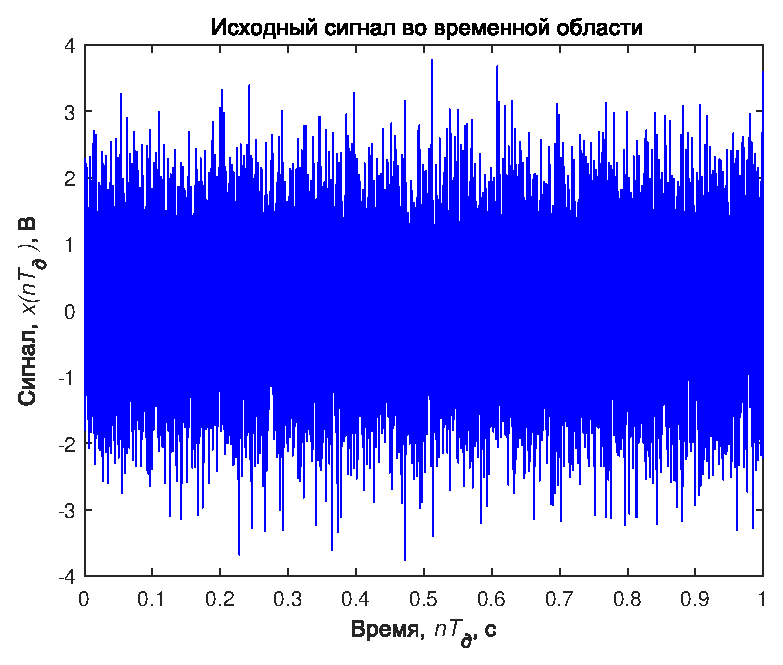
\includegraphics[width=\maxwidth{56.196688409433015em}]{figure_0}
\end{center}


\begin{par}
\begin{flushleft}
1.3 Построение амплитудного спектра белого шума
\end{flushleft}
\end{par}

\begin{matlabcode}
f = linspace(0, fd, N); % Формирование области определения в частотной области
% Массив отсчётов спектра исходного сигнала
fnoise = abs(fft(noise)/N);
figure; plot([-fliplr(f(1:end/2)) f(1:end/2)], fftshift(fnoise),...
    'Color', fColor, 'LineWidth', 3);
%axis([-fd/2 fd/2 0 volume*0.6]); % Диапазон значений осей
set(get(gcf, 'CurrentAxes'), 'FontSize', fontSize); % Изменение шрифта
title('\rm Исходный сигнал в частотной области'); % Заголовок
xlabel('Частота,\it f\rm, Гц'); % Надпись оси абсцисс
ylabel('Амплитуда,\it A(f)\rm, В'); % Надпись оси ординат
\end{matlabcode}
\begin{center}
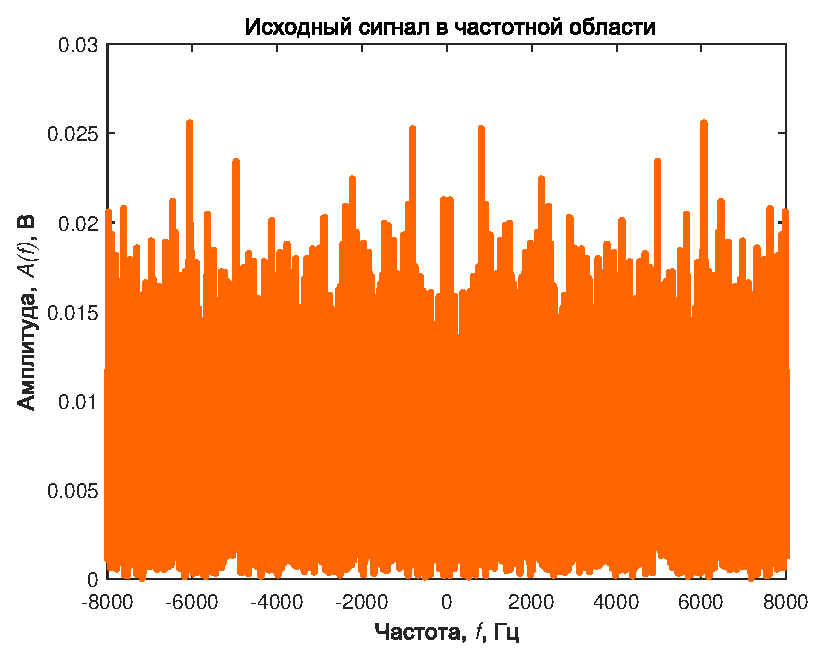
\includegraphics[width=\maxwidth{56.196688409433015em}]{figure_1}
\end{center}


\begin{par}
\begin{flushleft}
1.4 Создание режекторного фильтра в Matlab Filter Designer
\end{flushleft}
\end{par}

\begin{par}
\begin{flushleft}
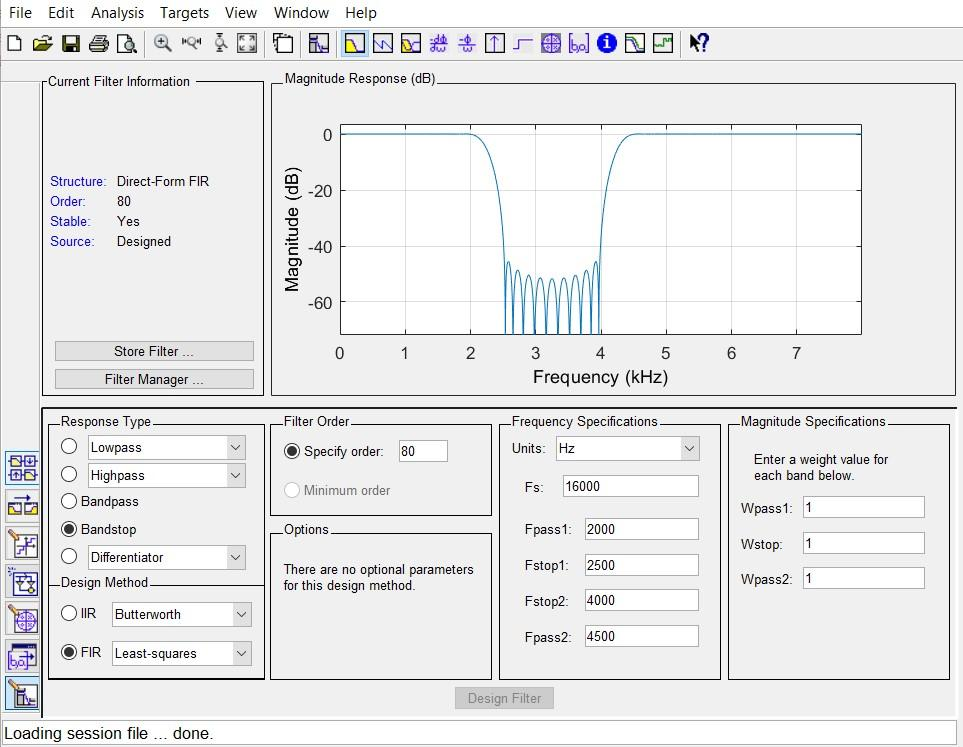
\includegraphics[width=\maxwidth{96.63823381836427em}]{image_0}
\end{flushleft}
\end{par}


\begin{par}
\begin{flushleft}
1.5 Экспорт коэффициентов фильтра в файл
\end{flushleft}
\end{par}

\begin{par}
\begin{flushleft}
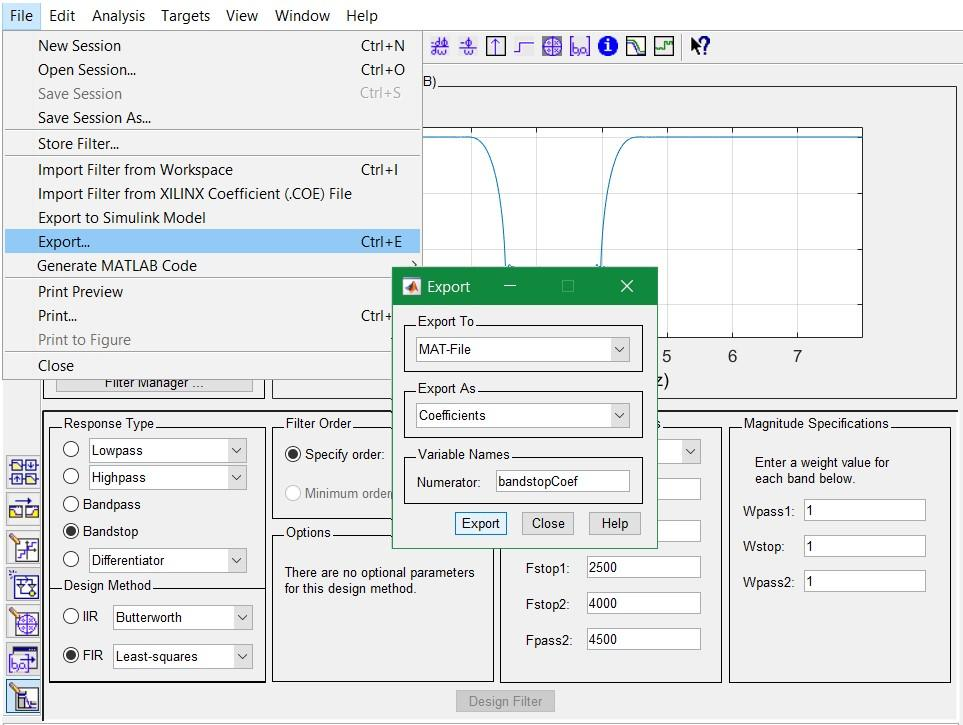
\includegraphics[width=\maxwidth{96.63823381836427em}]{image_1}
\end{flushleft}
\end{par}


\begin{par}
\begin{flushleft}
1.6 Фильтрация белого шума
\end{flushleft}
\end{par}

\begin{matlabcode}
load('bandstopFilter.mat'); % Загрузка файла с коэффициентами фильтра
global bandstopCoef; % Массив коэффициентов КИХ-фильтра
data = filter(bandstopCoef, 1, noise); % Применение фильтра к белому шуму
figure; plot(t, data, 'Color', tColor);
set(get(gcf, 'CurrentAxes'), 'FontSize', fontSize); % Изменение шрифта
title('\rm Отфильтрованный сигнал во временной области'); % Заголовок
xlabel('Время,\it nT_д\rm, с'); % Надпись оси абсцисс
ylabel('Сигнал,\it x(nT_д )\rm, В'); % Надпись оси ординат
\end{matlabcode}
\begin{center}
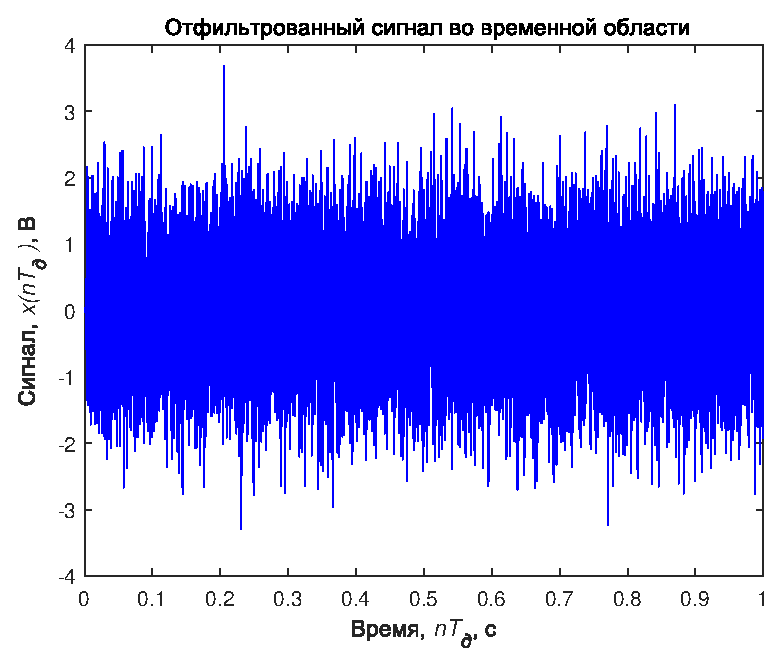
\includegraphics[width=\maxwidth{56.196688409433015em}]{figure_2}
\end{center}


\begin{par}
\begin{flushleft}
1.7 Построение амплитудного спектра отфильтрованного сигнала
\end{flushleft}
\end{par}

\begin{matlabcode}
% Массив отсчётов спектра отфильтрованного сигнала
fdata = abs(fft(data)/N);
figure; plot([-fliplr(f(1:end/2)) f(1:end/2)], fftshift(fdata),...
    'Color', fColor, 'LineWidth', 3);
%axis([-fd/2 fd/2 0 volume*0.6]); % Диапазон значений осей
set(get(gcf, 'CurrentAxes'), 'FontSize', fontSize); % Изменение шрифта
title('\rm Отфильтрованный сигнал в частотной области (АЧХ фильтра)'); % Заголовок
xlabel('Частота,\it f\rm, Гц'); % Надпись оси абсцисс
ylabel('Амплитуда,\it A(f)\rm, В'); % Надпись оси ординат
\end{matlabcode}
\begin{center}
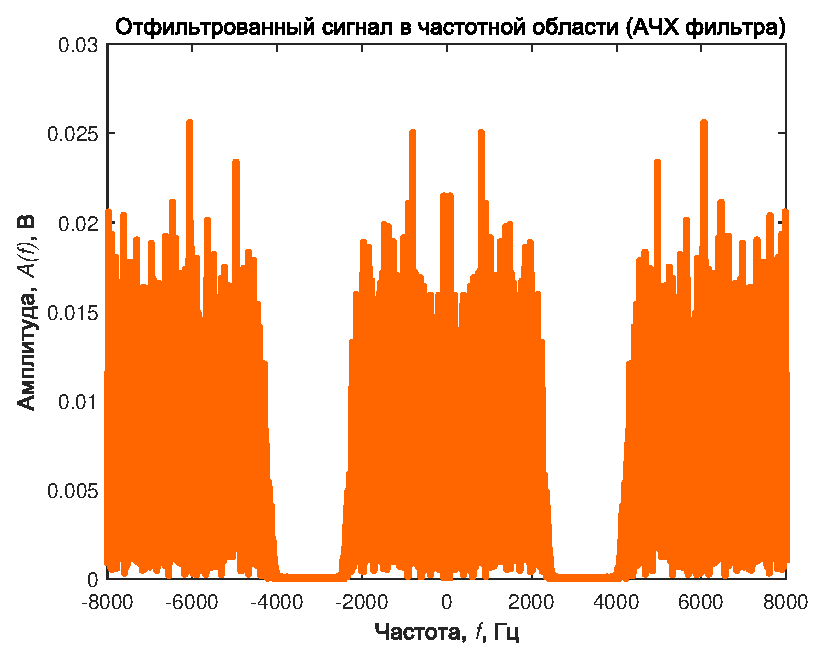
\includegraphics[width=\maxwidth{56.196688409433015em}]{figure_3}
\end{center}

\end{document}
